\begin{boxteo}Для абсолюно неперервного векторa $\begin{bmatrix}
	 \xi& \eta
	\end{bmatrix}^T$\\
$$\xi \independent \eta \Leftrightarrow f_{\xi, \eta} (x,y)= f_{\xi}(x) f_{\eta}(y) \quad \forall x,y \in \mathbb{R}$$
\end{boxteo}

\begin{proof}
$$
\begin{gathered}
1. \quad  F_{\xi, \eta} (x,y) = F_{\xi}(x) \cdot F_{\eta}(y) \Longrightarrow f_{\xi, \eta} (x,y) = f_{\xi}(x) \cdot f_{\eta}(y)\\
	2. \quad f_{\xi, \eta} (x,y) = f_{\xi}(x) \cdot f_{\eta}(y)\Longrightarrow F_{\xi, \eta} (x,y) = F_{\xi}(x) \cdot F_{\eta}(y)
\end{gathered}\quad \forall x,y \in \mathbb{R}
$$
2.
$$
F_{\xi, \eta} (x,y ) =  \int\limits_{-\infty}^{ x}{  \int\limits_{- \i}^{y}{ f_{\xi, \eta} (s,t) dsdt}} =  \int\limits_{- \i}^{ x}{  \int\limits_{-\i}^{y}{ f_{\xi} (s) \cdot f_{\eta} (t)dsdt}} =
$$
$$
= \int\limits_{-\i}^{ x}{ f_ \xi (s) ds}\cdot  \int\limits_{-\i}^{ +\infty}{f_\eta(t) dt} = F_{\xi}(s)\cdot F_{\eta}(t)
$$
1.
$$
f_{\xi, \eta} (x,y) = \frac{\partial^2 f}{\partial x \partial y} (x,y) = \frac{\d ^2}{\d x \d y} (F_{\xi}(x) \cdot F_{ \eta} (y) ) = \frac{\d}{\d x} (F_{\xi} (x) \cdot f_{\eta} (y) ) = f_{\xi}(x) \cdot f_{\eta}(y)
$$
\end{proof}

\subsection{Умовні розподіли та умовні математичні сподівання}

\subsubsection{Дискретний вектор}
$$
\begin{gathered}
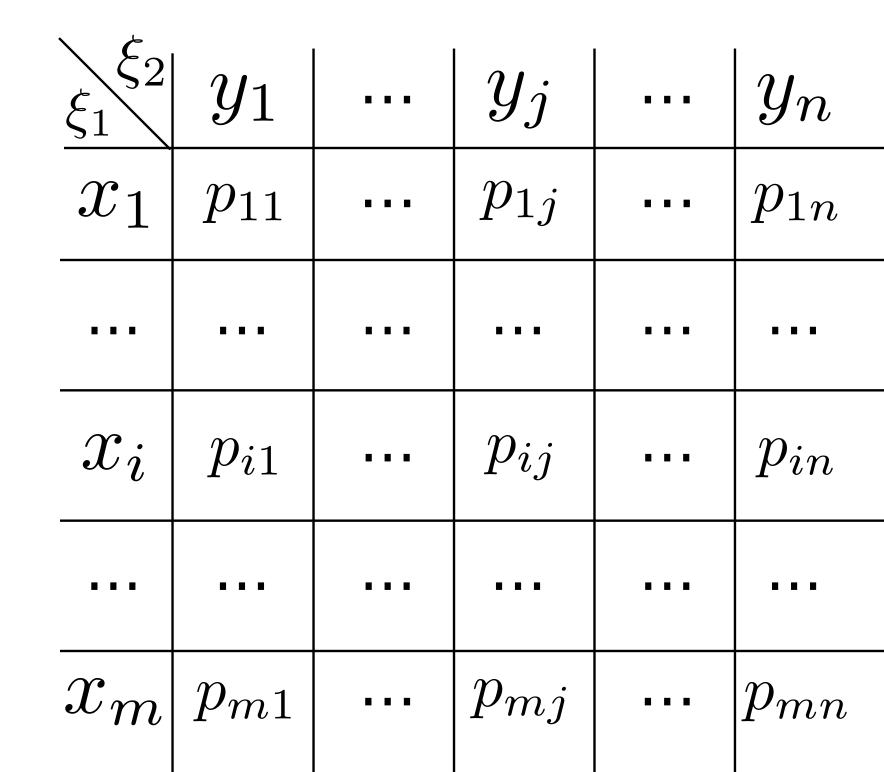
\includegraphics[scale=0.2]{images/14.png}
\end{gathered}\qquad\quad
\begin{gathered}
\text{Розподіли } \xi_2 \text{ за } \xi_1\\
\mathbb{P} \left\lbrace \xi_2 = y_j | \xi_2 = x_i \right\rbrace = \frac{\mathbb{P} \left\lbrace \xi_1 = x_i, \xi_2 = y_j \right\rbrace}{ \mathbb{P} \left\lbrace \xi_1 = x_i \right\rbrace} = \\
= \frac{p_{ij}}{  \sum\limits_{j = 1}^{n}{ p_ij}}
\end{gathered}
$$

\begin{center}
\textbf{Умовний ряд розподілу }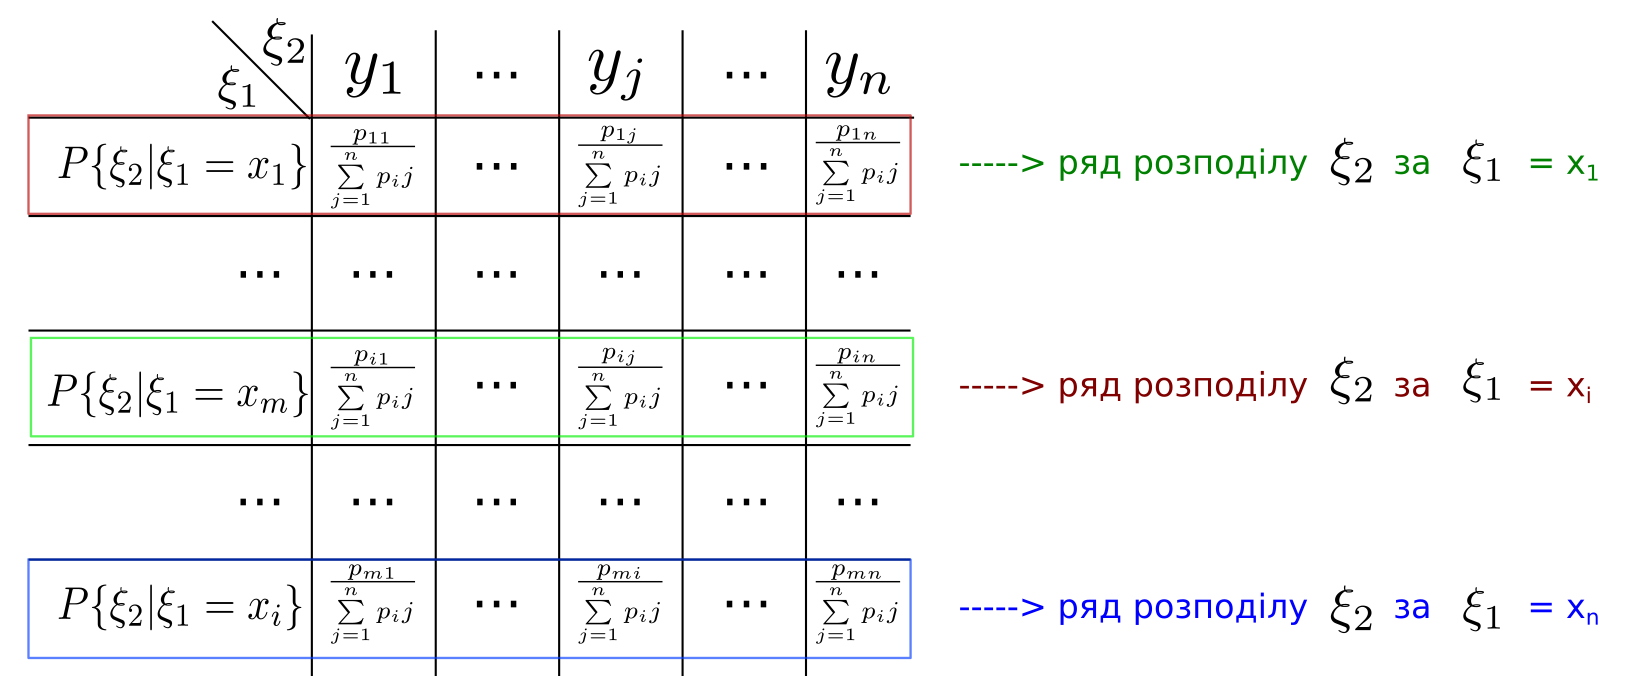
\includegraphics[scale=0.3]{images/20.png} \end{center}
$$
\mathbb{E}(\xi_2 | \xi_1 = x_i)  =  \sum\limits_{j = 1}^{ n}{ y_j \mathbb{P} \left\lbrace \xi_2 = y_j | \xi_1 = x_i \right\rbrace } =  \sum\limits_{j = 1}^{n}{ y_{j} \cdot \frac{p_{ij} }{  \sum\limits_{k = 1}^{ n}{p_{ik}}}}= \frac{  \sum\limits_{j = 1}^{ n}{ y_j p_{ij}}}{  \sum\limits_{j = 1}^{n}{ p_{ij}}}
$$
$$
\begin{matrix}
	\xi_1 & x_1 & \cdots  &x_i & \cdots & x_m \\
	\mathbb{E}_{\xi_2 | \xi_1=x_k}  &  \frac{  \sum\limits_{j = 1}^{ n}{ y_j p_{1j}}}{  \sum\limits_{j = 1}^{n}{ p_{1j}}}  & \cdots  &\frac{  \sum\limits_{j = 1}^{ n}{ y_j p_{ij}}}{  \sum\limits_{j = 1}^{n}{ p_{ij}}}  & \cdots & \frac{  \sum\limits_{j = 1}^{ n}{ y_j p_{mj}}}{  \sum\limits_{j = 1}^{n}{ p_{mj}}}  \\
	\mathbb{P} \left\lbrace \xi_1 = x_k \right\rbrace &   \sum\limits_{j = 1}^{n}{ p_{ij}} & \cdots  &\sum\limits_{j = 1}^{n}{ p_{ij}} & \cdots & \sum\limits_{j = 1}^{n}{ p_{mj}} \\
\end{matrix}
\begin{gathered}
\longrightarrow \text{ряд розподілу}\\
\mathbb{E}(\xi_2| \xi_1)
\end{gathered}
$$
$
\mathbb{E} (\xi_2 | \xi_1)
$ - умовне математичне сподівання $\xi_2$ за умови, що $\xi_1$ набула деяке своє значення $(x_1 \lor x_2 \lor ... \lor x_m)$
\begin{center}
	Формула повного математичного сподівання
\end{center}
$$
\mathbb{E}[ \mathbb{E} (\xi_2 | \xi_1)] =
\frac{  \sum\limits_{j = 1}^{n}  {y_j \cdot p_{1j}} }   {  \sum\limits_{j = 1}^{ n}{ p_{1j}}} \cdot  \sum\limits_{j = 1}^{ n}{ p_{1j}}+ ... +
\frac{  \sum\limits_{j = 1}^{n}{y_j \cdot p_{mj}} }   {  \sum\limits_{j = 1}^{ n}{ p_{mj}}} \cdot  \sum\limits_{j = 1}^{ n}{ p_{mj}} =  \sum\limits_{i = 1}^{m}{  \sum\limits_{j =1 }^{ n}{ y_j p_{ij}}} = \mathbb{E}\xi_2
$$
$$
\mathbb{E}[ \mathbb{E} (\xi_2 | \xi_1)] = \mathbb{E}  \xi_2  \quad \quad \quad \mathbb{E}[ \mathbb{E} (\xi_1 | \xi_2)] = \mathbb{E}  \xi_1
$$
\subsubsection{Абсолютно неперервний вектор}
$$
\overline{\xi}  \begin{bmatrix}
 \xi_1 \\ \xi_2
\end{bmatrix} \qquad f_{\overline{\xi}} (x,y) - \text{ сумісна щільність розподілу.}
$$
$
f_{\xi_2 | \xi_1} (y|y) = f_{\xi_2| \xi_1 = x} (y)
$ - умовна щільність другої координати за першою.\\

$F_{\xi_2 | \xi_1 = x} (y)$ - умовна функція розподілу $\xi_2$ за умови $\xi_1 = x$.\\
$ F_{\xi_2 | \xi_1 = x} (y) = \mathbb{P} \left\lbrace \xi_2 < y | \xi_1 = x  \right\rbrace = \frac{\mathbb{P} \left\lbrace \xi_1  = x , \xi_2 < y \right\rbrace}{ \mathbb{P} \left\lbrace \xi_1 = x \right\rbrace} = \frac{0}{0} $
\\$$   F_{\xi_2 | \xi_1 = x} (y) = \lim\limits_{\varepsilon \to  \infty}{
 \mathbb{P} \left\lbrace  \xi_2 | \xi_1 \in [x, x+ \varepsilon ) \right\rbrace
 } =  \frac{ \mathbb{P} \left\lbrace \xi_1 \in [x, x+ \varepsilon ) , \xi_2 \in (- \i, y)\right\rbrace}{ \mathbb{P} \left\lbrace \xi_1 \in [x, x + \varepsilon ) \right\rbrace} =
  $$
	$$
	=  \lim\limits_{\varepsilon \to  0} { \frac{\int\limits_{x}^{ x+\varepsilon }{ ds  \int\limits_{- \i}^{ y}{ f_{ \overline{\xi}}}(s,t)dt}}{
  \int\limits_{x}^{ x+\varepsilon }{ f_{\xi_1} (s) ds}}
  } =    \lim\limits_{\varepsilon \to  0} { \frac{\varepsilon \cdot\int\limits_{x}^{ x+\varepsilon }{ ds  \int\limits_{- \i}^{ y}{ f_{ \overline{\xi}}}(s,t)dt}}{ \varepsilon \cdot
  \int\limits_{x}^{ x+\varepsilon }{  f_{\xi_1} (s) ds}}
  }  =  \fbox{$ \displaystyle\frac{  \int\limits_{- \i}^{ y}{ f_{ \overline{\xi}} }(x,t)dt}{ f_{\xi_1} (x)} = F_{\xi_2 | \xi_1 = x} (y)$}
	$$
Знаючи умовну функцію розподілу, можемо знайти умовну щільність:
	$$
	f_{\xi_2 | \xi_1 = x} = F_{\xi_2| \xi_1 = x}'(y) = \frac{f_{\overline{\xi}}(x,y)}{ f_{\xi_1}(x)}
	$$
Знайдемо умовне математичне сподівання $\xi_2$ за $\xi_1$
	$$
	\mathbb{E}(\xi_2 | \xi_1 = x) =  \int\limits_{-\i}^{ +\infty}{ y \cdot f_{\xi_2 | \xi_1 = x} dy} =  \int\limits_{-\i}^{ +\infty}{ y \cdot \frac{f_{\overline{\xi}}(x,y)}{ f_{\xi_1} (x)}  dy} =
	\frac{
	\int\limits_{-\i}^{ +\infty}{ y \cdot f_{\overline{\xi}}(x,y)}dy}{ f_{\xi_1} (x)}
	$$
$ \mathbb{E} (\xi_2| \xi_1)$ - випадкова величина, яка спочатку визначає, куди попала умова (чому дорівнює $x \longleftarrow \xi_1$), а далі визначає $\mathbb{E}(\xi_2| \xi_1 = x)$.\\
$\mathbb{E}(\xi_2| \xi_1)$ - набуває значення $ \mathbb{E}(\xi_2 | \xi_1 = x)$, коли $\xi_1$ набула значення $x$.
$$\xi_1 \longrightarrow x \Rightarrow \mathbb{E}(\xi_2 | \xi_1) \longrightarrow \mathbb{E}(\xi_2 | \xi_1 = x)$$
$ \mathbb{E}(\xi_2 | \xi_1)$ є функцією від $\xi_1$. Якою? $ \mathbb{E}(\xi_2 | \xi_1 = x)$\\
$ \mathbb{E} (\xi_2 | \xi_1 ) = \Psi (\xi_1)$, де $ \Psi(x) = \mathbb{E}( \xi_2 | \xi_1 = x)$
